\documentclass[border=3pt,tikz]{standalone}
\usepackage{amsmath}
\begin{document}
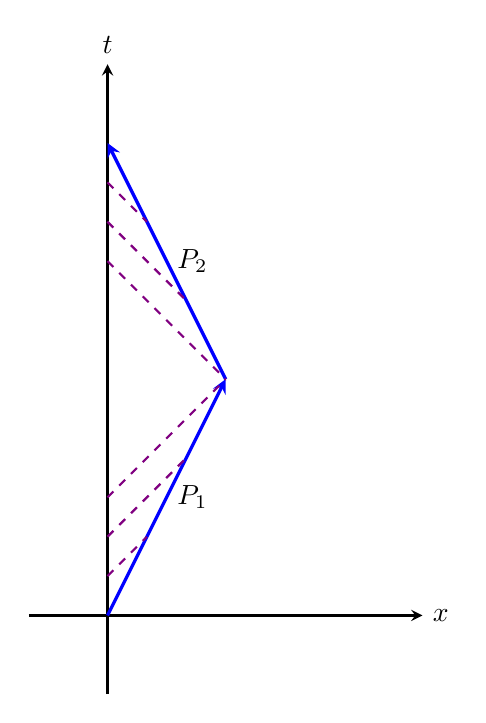
\begin{tikzpicture}[]
    \draw[thick,->,>=stealth] (0, -1) -- (0, 7) node[above] {$t$};
    \draw[thick,->,>=stealth] (-1, 0) -- (4, 0) node[right] {$x$};
    \draw[very thick, blue, ->,>=stealth] (0,0) --(0.75, 1.5) node[right, black] {$P_1$}-- (1.5, 3);
    \draw[very thick, blue, ->,>=stealth] (1.5, 3) --(0.75, 4.5) node[right, black] {$P_2$}-- (0, 6);
    % \draw[red, dashed] (0,0)-- (4, 4) node[right] {$x=ct$};
    \draw[thick, violet, dashed](0, 0.5) -- (0.5, 1);
    \draw[thick, violet, dashed](0, 1) -- (1, 2);
    \draw[thick, violet, dashed](0, 1.5) -- (1.5, 3);
    \draw[thick, violet, dashed](0, 4.5) -- (1.5, 3);
    \draw[thick, violet, dashed](0, 5) -- (1, 4);
    \draw[thick, violet, dashed](0, 5.5) -- (0.5, 5);
    \end{tikzpicture}

\end{document}